% Graphic for TeX using PGF
% Title: C:\Users\Nicolas Chicaiza\Dia\arbolProblemas.dia
% Creator: Dia v0.97.2
% CreationDate: Sun May 02 21:05:28 2021
% For: Nicolas Chicaiza
% \usepackage{tikz}
% The following commands are not supported in PSTricks at present
% We define them conditionally, so when they are implemented,
% this pgf file will use them.
\definecolor{titulo}{RGB}{41,56,69}
\begin{figure}[H]
    \centering
    \ifx\du\undefined
    \newlength{\du}
    \fi
    \setlength{\du}{15\unitlength}
    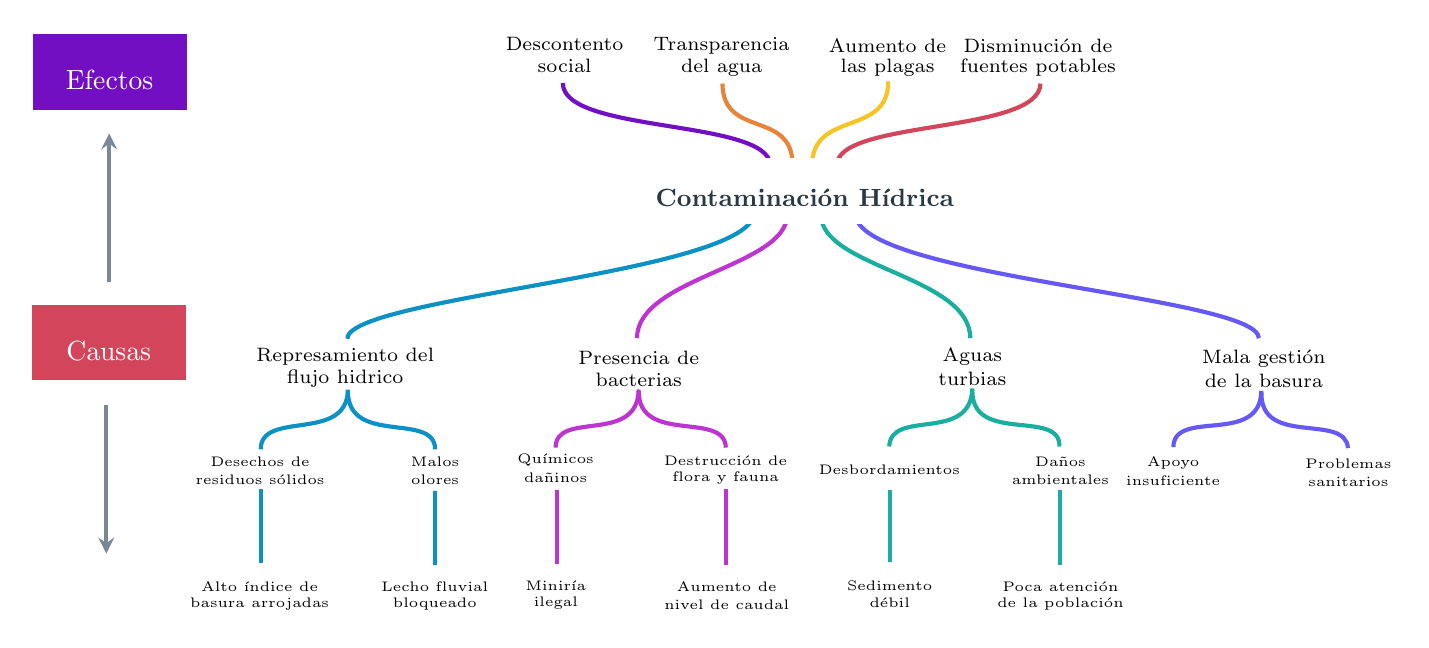
\begin{tikzpicture}
        \pgftransformxscale{1.000000}
        \pgftransformyscale{-1.000000}
        \definecolor{dialinecolor}{rgb}{0.000000, 0.000000, 0.000000}
        \pgfsetstrokecolor{dialinecolor}
        \definecolor{dialinecolor}{rgb}{1.000000, 1.000000, 1.000000}
        \pgfsetfillcolor{dialinecolor}
        \pgfsetlinewidth{0.100000\du}
        \pgfsetdash{}{0pt}
        \pgfsetdash{}{0pt}
        \pgfsetmiterjoin
        \pgfsetbuttcap
        {
        \definecolor{dialinecolor}{rgb}{0.101961, 0.682353, 0.623529}
        \pgfsetfillcolor{dialinecolor}
        % was here!!!
        \definecolor{dialinecolor}{rgb}{0.101961, 0.682353, 0.623529}
        \pgfsetstrokecolor{dialinecolor}
        \pgfpathmoveto{\pgfpoint{37.405868\du}{11.384334\du}}
        \pgfpathcurveto{\pgfpoint{37.394405\du}{12.662399\du}}{\pgfpoint{41.001828\du}{12.864948\du}}{\pgfpoint{41.001828\du}{14.364948\du}}
        \pgfusepath{stroke}
        }
        \pgfsetlinewidth{0.100000\du}
        \pgfsetdash{}{0pt}
        \pgfsetdash{}{0pt}
        \pgfsetmiterjoin
        \pgfsetbuttcap
        {
        \definecolor{dialinecolor}{rgb}{0.741176, 0.203922, 0.819608}
        \pgfsetfillcolor{dialinecolor}
        % was here!!!
        \definecolor{dialinecolor}{rgb}{0.741176, 0.203922, 0.819608}
        \pgfsetstrokecolor{dialinecolor}
        \pgfpathmoveto{\pgfpoint{36.592704\du}{11.384334\du}}
        \pgfpathcurveto{\pgfpoint{36.593868\du}{12.642708\du}}{\pgfpoint{32.973106\du}{12.903483\du}}{\pgfpoint{32.973106\du}{14.364948\du}}
        \pgfusepath{stroke}
        }
        \pgfsetlinewidth{0.100000\du}
        \pgfsetdash{}{0pt}
        \pgfsetdash{}{0pt}
        \pgfsetmiterjoin
        \pgfsetbuttcap
        {
        \definecolor{dialinecolor}{rgb}{0.047059, 0.568627, 0.772549}
        \pgfsetfillcolor{dialinecolor}
        % was here!!!
        \definecolor{dialinecolor}{rgb}{0.047059, 0.568627, 0.772549}
        \pgfsetstrokecolor{dialinecolor}
        \pgfpathmoveto{\pgfpoint{35.797217\du}{11.331302\du}}
        \pgfpathcurveto{\pgfpoint{35.785755\du}{12.804229\du}}{\pgfpoint{25.993979\du}{13.359000\du}}{\pgfpoint{25.993979\du}{14.378579\du}}
        \pgfusepath{stroke}
        }
        % setfont left to latex
        \definecolor{dialinecolor}{rgb}{0.000000, 0.000000, 0.000000}
        \pgfsetstrokecolor{dialinecolor}
        \node at (25.942974\du,14.815404\du){\scriptsize Represamiento del};
        % setfont left to latex
        \definecolor{dialinecolor}{rgb}{0.000000, 0.000000, 0.000000}
        \pgfsetstrokecolor{dialinecolor}
        \node at (25.942974\du,15.344571\du){\scriptsize flujo hidrico};
        % setfont left to latex
        \definecolor{dialinecolor}{rgb}{0.000000, 0.000000, 0.000000}
        \pgfsetstrokecolor{dialinecolor}
        \node[anchor=west] at (24.709536\du,16.205230\du){};
        % setfont left to latex
        \definecolor{dialinecolor}{rgb}{0.000000, 0.000000, 0.000000}
        \pgfsetstrokecolor{dialinecolor}
        \node[anchor=west] at (37.027529\du,10.825328\du){};
        \pgfsetlinewidth{0.100000\du}
        \pgfsetdash{}{0pt}
        \pgfsetdash{}{0pt}
        \pgfsetmiterjoin
        \pgfsetbuttcap
        {
        \definecolor{dialinecolor}{rgb}{0.047059, 0.568627, 0.772549}
        \pgfsetfillcolor{dialinecolor}
        % was here!!!
        \definecolor{dialinecolor}{rgb}{0.047059, 0.568627, 0.772549}
        \pgfsetstrokecolor{dialinecolor}
        \pgfpathmoveto{\pgfpoint{26.009356\du}{15.642044\du}}
        \pgfpathcurveto{\pgfpoint{26.008024\du}{16.967970\du}}{\pgfpoint{28.110242\du}{16.127083\du}}{\pgfpoint{28.109356\du}{17.042044\du}}
        \pgfusepath{stroke}
        }
        \pgfsetlinewidth{0.100000\du}
        \pgfsetdash{}{0pt}
        \pgfsetdash{}{0pt}
        \pgfsetmiterjoin
        \pgfsetbuttcap
        {
        \definecolor{dialinecolor}{rgb}{0.047059, 0.568627, 0.772549}
        \pgfsetfillcolor{dialinecolor}
        % was here!!!
        \definecolor{dialinecolor}{rgb}{0.047059, 0.568627, 0.772549}
        \pgfsetstrokecolor{dialinecolor}
        \pgfpathmoveto{\pgfpoint{26.007805\du}{15.603965\du}}
        \pgfpathcurveto{\pgfpoint{25.997513\du}{16.894392\du}}{\pgfpoint{23.905806\du}{16.085038\du}}{\pgfpoint{23.909356\du}{17.042044\du}}
        \pgfusepath{stroke}
        }
        % setfont left to latex
        \definecolor{dialinecolor}{rgb}{0.000000, 0.000000, 0.000000}
        \pgfsetstrokecolor{dialinecolor}
        \node at (23.893734\du,17.351322\du){\tiny Desechos de};
        % setfont left to latex
        \definecolor{dialinecolor}{rgb}{0.000000, 0.000000, 0.000000}
        \pgfsetstrokecolor{dialinecolor}
        \node at (23.893734\du,17.774655\du){\tiny residuos sólidos};
        % setfont left to latex
        \definecolor{dialinecolor}{rgb}{0.000000, 0.000000, 0.000000}
        \pgfsetstrokecolor{dialinecolor}
        \node at (28.109356\du,17.346702\du){\tiny Malos};
        % setfont left to latex
        \definecolor{dialinecolor}{rgb}{0.000000, 0.000000, 0.000000}
        \pgfsetstrokecolor{dialinecolor}
        \node at (28.109356\du,17.770035\du){\tiny olores};
        % setfont left to latex
        \definecolor{dialinecolor}{rgb}{0.000000, 0.000000, 0.000000}
        \pgfsetstrokecolor{dialinecolor}
        \node at (33.015835\du,14.833847\du){\scriptsize Presencia de};
        % setfont left to latex
        \definecolor{dialinecolor}{rgb}{0.000000, 0.000000, 0.000000}
        \pgfsetstrokecolor{dialinecolor}
        \node at (33.015835\du,15.363014\du){\scriptsize bacterias};
        \pgfsetlinewidth{0.100000\du}
        \pgfsetdash{}{0pt}
        \pgfsetdash{}{0pt}
        \pgfsetmiterjoin
        \pgfsetbuttcap
        {
        \definecolor{dialinecolor}{rgb}{0.741176, 0.203922, 0.819608}
        \pgfsetfillcolor{dialinecolor}
        % was here!!!
        \definecolor{dialinecolor}{rgb}{0.741176, 0.203922, 0.819608}
        \pgfsetstrokecolor{dialinecolor}
        \pgfpathmoveto{\pgfpoint{33.014808\du}{15.638079\du}}
        \pgfpathcurveto{\pgfpoint{33.008410\du}{16.936437\du}}{\pgfpoint{35.089606\du}{16.106061\du}}{\pgfpoint{35.113256\du}{17.000000\du}}
        \pgfusepath{stroke}
        }
        \pgfsetlinewidth{0.100000\du}
        \pgfsetdash{}{0pt}
        \pgfsetdash{}{0pt}
        \pgfsetmiterjoin
        \pgfsetbuttcap
        {
        \definecolor{dialinecolor}{rgb}{0.741176, 0.203922, 0.819608}
        \pgfsetfillcolor{dialinecolor}
        % was here!!!
        \definecolor{dialinecolor}{rgb}{0.741176, 0.203922, 0.819608}
        \pgfsetstrokecolor{dialinecolor}
        \pgfpathmoveto{\pgfpoint{33.013256\du}{15.600000\du}}
        \pgfpathcurveto{\pgfpoint{32.997899\du}{16.936437\du}}{\pgfpoint{31.011303\du}{16.095550\du}}{\pgfpoint{31.013256\du}{17.000000\du}}
        \pgfusepath{stroke}
        }
        % setfont left to latex
        \definecolor{dialinecolor}{rgb}{0.000000, 0.000000, 0.000000}
        \pgfsetstrokecolor{dialinecolor}
        \node[anchor=west] at (31.800000\du,14.800000\du){};
        % setfont left to latex
        \definecolor{dialinecolor}{rgb}{0.000000, 0.000000, 0.000000}
        \pgfsetstrokecolor{dialinecolor}
        \node[anchor=west] at (30.800000\du,15.000000\du){};
        % setfont left to latex
        \definecolor{dialinecolor}{rgb}{0.000000, 0.000000, 0.000000}
        \pgfsetstrokecolor{dialinecolor}
        \node[anchor=west] at (32.000000\du,15.000000\du){};
        % setfont left to latex
        \definecolor{dialinecolor}{rgb}{0.000000, 0.000000, 0.000000}
        \pgfsetstrokecolor{dialinecolor}
        \node[anchor=west] at (32.600000\du,15.200000\du){};
        % setfont left to latex
        \definecolor{dialinecolor}{rgb}{0.000000, 0.000000, 0.000000}
        \pgfsetstrokecolor{dialinecolor}
        \node[anchor=west] at (31.400000\du,14.600000\du){};
        % setfont left to latex
        \definecolor{dialinecolor}{rgb}{0.000000, 0.000000, 0.000000}
        \pgfsetstrokecolor{dialinecolor}
        \node at (31.013256\du,17.309847\du){\tiny Químicos};
        % setfont left to latex
        \definecolor{dialinecolor}{rgb}{0.000000, 0.000000, 0.000000}
        \pgfsetstrokecolor{dialinecolor}
        \node at (31.013256\du,17.733181\du){\tiny dañinos};
        % setfont left to latex
        \definecolor{dialinecolor}{rgb}{0.000000, 0.000000, 0.000000}
        \pgfsetstrokecolor{dialinecolor}
        \node at (35.107016\du,17.319207\du){\tiny Destrucción de};
        % setfont left to latex
        \definecolor{dialinecolor}{rgb}{0.000000, 0.000000, 0.000000}
        \pgfsetstrokecolor{dialinecolor}
        \node at (35.107016\du,17.742541\du){\tiny flora y fauna};
        \pgfsetlinewidth{0.100000\du}
        \pgfsetdash{}{0pt}
        \pgfsetdash{}{0pt}
        \pgfsetmiterjoin
        \pgfsetbuttcap
        {
        \definecolor{dialinecolor}{rgb}{0.396078, 0.345098, 0.960784}
        \pgfsetfillcolor{dialinecolor}
        % was here!!!
        \definecolor{dialinecolor}{rgb}{0.396078, 0.345098, 0.960784}
        \pgfsetstrokecolor{dialinecolor}
        \pgfpathmoveto{\pgfpoint{38.236709\du}{11.348979\du}}
        \pgfpathcurveto{\pgfpoint{38.156472\du}{12.896409\du}}{\pgfpoint{47.953693\du}{13.345369\du}}{\pgfpoint{47.953693\du}{14.364948\du}}
        \pgfusepath{stroke}
        }
        % setfont left to latex
        \definecolor{dialinecolor}{rgb}{0.000000, 0.000000, 0.000000}
        \pgfsetstrokecolor{dialinecolor}
        \node at (48.074411\du,14.857680\du){\scriptsize Mala gestión};
        % setfont left to latex
        \definecolor{dialinecolor}{rgb}{0.000000, 0.000000, 0.000000}
        \pgfsetstrokecolor{dialinecolor}
        \node at (48.074411\du,15.386846\du){\scriptsize de la basura};
        % setfont left to latex
        \definecolor{dialinecolor}{rgb}{0.000000, 0.000000, 0.000000}
        \pgfsetstrokecolor{dialinecolor}
        \node[anchor=west] at (46.647799\du,16.368816\du){};
        \pgfsetlinewidth{0.100000\du}
        \pgfsetdash{}{0pt}
        \pgfsetdash{}{0pt}
        \pgfsetmiterjoin
        \pgfsetbuttcap
        {
        \definecolor{dialinecolor}{rgb}{0.396078, 0.345098, 0.960784}
        \pgfsetfillcolor{dialinecolor}
        % was here!!!
        \definecolor{dialinecolor}{rgb}{0.396078, 0.345098, 0.960784}
        \pgfsetstrokecolor{dialinecolor}
        \pgfpathmoveto{\pgfpoint{48.015090\du}{15.670689\du}}
        \pgfpathcurveto{\pgfpoint{47.985360\du}{16.993676\du}}{\pgfpoint{50.032213\du}{16.151419\du}}{\pgfpoint{50.100988\du}{17.011102\du}}
        \pgfusepath{stroke}
        }
        \pgfsetlinewidth{0.100000\du}
        \pgfsetdash{}{0pt}
        \pgfsetdash{}{0pt}
        \pgfsetmiterjoin
        \pgfsetbuttcap
        {
        \definecolor{dialinecolor}{rgb}{0.396078, 0.345098, 0.960784}
        \pgfsetfillcolor{dialinecolor}
        % was here!!!
        \definecolor{dialinecolor}{rgb}{0.396078, 0.345098, 0.960784}
        \pgfsetstrokecolor{dialinecolor}
        \pgfpathmoveto{\pgfpoint{48.013539\du}{15.632609\du}}
        \pgfpathcurveto{\pgfpoint{47.991899\du}{16.965252\du}}{\pgfpoint{45.905734\du}{16.048257\du}}{\pgfpoint{45.894272\du}{16.988177\du}}
        \pgfusepath{stroke}
        }
        % setfont left to latex
        \definecolor{dialinecolor}{rgb}{0.000000, 0.000000, 0.000000}
        \pgfsetstrokecolor{dialinecolor}
        \node at (45.888757\du,17.371821\du){\tiny Apoyo};
        % setfont left to latex
        \definecolor{dialinecolor}{rgb}{0.000000, 0.000000, 0.000000}
        \pgfsetstrokecolor{dialinecolor}
        \node at (45.888757\du,17.795155\du){\tiny insuficiente};
        % setfont left to latex
        \definecolor{dialinecolor}{rgb}{0.000000, 0.000000, 0.000000}
        \pgfsetstrokecolor{dialinecolor}
        \node at (50.112057\du,17.399769\du){\tiny Problemas};
        % setfont left to latex
        \definecolor{dialinecolor}{rgb}{0.000000, 0.000000, 0.000000}
        \pgfsetstrokecolor{dialinecolor}
        \node at (50.112057\du,17.823102\du){\tiny sanitarios};
        % setfont left to latex
        \definecolor{dialinecolor}{rgb}{0.000000, 0.000000, 0.000000}
        \pgfsetstrokecolor{dialinecolor}
        \node at (41.052593\du,14.807772\du){\scriptsize Aguas};
        % setfont left to latex
        \definecolor{dialinecolor}{rgb}{0.000000, 0.000000, 0.000000}
        \pgfsetstrokecolor{dialinecolor}
        \node at (41.052593\du,15.336939\du){\scriptsize turbias};
        \pgfsetlinewidth{0.100000\du}
        \pgfsetdash{}{0pt}
        \pgfsetdash{}{0pt}
        \pgfsetmiterjoin
        \pgfsetbuttcap
        {
        \definecolor{dialinecolor}{rgb}{0.101961, 0.682353, 0.623529}
        \pgfsetfillcolor{dialinecolor}
        % was here!!!
        \definecolor{dialinecolor}{rgb}{0.101961, 0.682353, 0.623529}
        \pgfsetstrokecolor{dialinecolor}
        \pgfpathmoveto{\pgfpoint{41.051566\du}{15.612004\du}}
        \pgfpathcurveto{\pgfpoint{41.021836\du}{16.934992\du}}{\pgfpoint{43.179744\du}{16.052293\du}}{\pgfpoint{43.150014\du}{16.973925\du}}
        \pgfusepath{stroke}
        }
        \pgfsetlinewidth{0.100000\du}
        \pgfsetdash{}{0pt}
        \pgfsetdash{}{0pt}
        \pgfsetmiterjoin
        \pgfsetbuttcap
        {
        \definecolor{dialinecolor}{rgb}{0.101961, 0.682353, 0.623529}
        \pgfsetfillcolor{dialinecolor}
        % was here!!!
        \definecolor{dialinecolor}{rgb}{0.101961, 0.682353, 0.623529}
        \pgfsetstrokecolor{dialinecolor}
        \pgfpathmoveto{\pgfpoint{41.050014\du}{15.573925\du}}
        \pgfpathcurveto{\pgfpoint{41.020284\du}{16.896912\du}}{\pgfpoint{39.079744\du}{16.052293\du}}{\pgfpoint{39.050014\du}{16.973925\du}}
        \pgfusepath{stroke}
        }
        % setfont left to latex
        \definecolor{dialinecolor}{rgb}{0.000000, 0.000000, 0.000000}
        \pgfsetstrokecolor{dialinecolor}
        \node at (39.053553\du,17.532319\du){\tiny Desbordamientos};
        % setfont left to latex
        \definecolor{dialinecolor}{rgb}{0.000000, 0.000000, 0.000000}
        \pgfsetstrokecolor{dialinecolor}
        \node at (43.175107\du,17.346439\du){\tiny Daños};
        % setfont left to latex
        \definecolor{dialinecolor}{rgb}{0.000000, 0.000000, 0.000000}
        \pgfsetstrokecolor{dialinecolor}
        \node at (43.175107\du,17.769773\du){\tiny ambientales};
        \pgfsetlinewidth{0.100000\du}
        \pgfsetdash{}{0pt}
        \pgfsetdash{}{0pt}
        \pgfsetbuttcap
        {
        \definecolor{dialinecolor}{rgb}{0.047059, 0.568627, 0.772549}
        \pgfsetfillcolor{dialinecolor}
        % was here!!!
        \definecolor{dialinecolor}{rgb}{0.047059, 0.568627, 0.772549}
        \pgfsetstrokecolor{dialinecolor}
        \draw (23.908419\du,17.990822\du)--(23.908419\du,19.790129\du);
        }
        \pgfsetlinewidth{0.100000\du}
        \pgfsetdash{}{0pt}
        \pgfsetdash{}{0pt}
        \pgfsetbuttcap
        {
        \definecolor{dialinecolor}{rgb}{0.047059, 0.568627, 0.772549}
        \pgfsetfillcolor{dialinecolor}
        % was here!!!
        \definecolor{dialinecolor}{rgb}{0.047059, 0.568627, 0.772549}
        \pgfsetstrokecolor{dialinecolor}
        \draw (28.106801\du,18.045347\du)--(28.106801\du,19.817391\du);
        }
        % setfont left to latex
        \definecolor{dialinecolor}{rgb}{0.000000, 0.000000, 0.000000}
        \pgfsetstrokecolor{dialinecolor}
        \node at (23.883028\du,20.347956\du){\tiny Alto índice de };
        % setfont left to latex
        \definecolor{dialinecolor}{rgb}{0.000000, 0.000000, 0.000000}
        \pgfsetstrokecolor{dialinecolor}
        \node at (23.883028\du,20.771289\du){\tiny basura arrojadas};
        % setfont left to latex
        \definecolor{dialinecolor}{rgb}{0.000000, 0.000000, 0.000000}
        \pgfsetstrokecolor{dialinecolor}
        \node at (28.103020\du,20.340299\du){\tiny Lecho fluvial};
        % setfont left to latex
        \definecolor{dialinecolor}{rgb}{0.000000, 0.000000, 0.000000}
        \pgfsetstrokecolor{dialinecolor}
        \node at (28.103020\du,20.763632\du){\tiny bloqueado};
        \pgfsetlinewidth{0.100000\du}
        \pgfsetdash{}{0pt}
        \pgfsetdash{}{0pt}
        \pgfsetbuttcap
        {
        \definecolor{dialinecolor}{rgb}{0.741176, 0.203922, 0.819608}
        \pgfsetfillcolor{dialinecolor}
        % was here!!!
        \definecolor{dialinecolor}{rgb}{0.741176, 0.203922, 0.819608}
        \pgfsetstrokecolor{dialinecolor}
        \draw (31.037489\du,18.018085\du)--(31.037489\du,19.803760\du);
        }
        \pgfsetlinewidth{0.100000\du}
        \pgfsetdash{}{0pt}
        \pgfsetdash{}{0pt}
        \pgfsetbuttcap
        {
        \definecolor{dialinecolor}{rgb}{0.741176, 0.203922, 0.819608}
        \pgfsetfillcolor{dialinecolor}
        % was here!!!
        \definecolor{dialinecolor}{rgb}{0.741176, 0.203922, 0.819608}
        \pgfsetstrokecolor{dialinecolor}
        \draw (35.126821\du,18.004453\du)--(35.126821\du,19.817391\du);
        }
        % setfont left to latex
        \definecolor{dialinecolor}{rgb}{0.000000, 0.000000, 0.000000}
        \pgfsetstrokecolor{dialinecolor}
        \node at (31.020337\du,20.330066\du){\tiny Miniría};
        % setfont left to latex
        \definecolor{dialinecolor}{rgb}{0.000000, 0.000000, 0.000000}
        \pgfsetstrokecolor{dialinecolor}
        \node at (31.020337\du,20.753400\du){\tiny ilegal};
        % setfont left to latex
        \definecolor{dialinecolor}{rgb}{0.000000, 0.000000, 0.000000}
        \pgfsetstrokecolor{dialinecolor}
        \node at (35.135218\du,20.353942\du){\tiny Aumento de};
        % setfont left to latex
        \definecolor{dialinecolor}{rgb}{0.000000, 0.000000, 0.000000}
        \pgfsetstrokecolor{dialinecolor}
        \node at (35.135218\du,20.777276\du){\tiny nivel de caudal};
        \pgfsetlinewidth{0.100000\du}
        \pgfsetdash{}{0pt}
        \pgfsetdash{}{0pt}
        \pgfsetbuttcap
        {
        \definecolor{dialinecolor}{rgb}{0.101961, 0.682353, 0.623529}
        \pgfsetfillcolor{dialinecolor}
        % was here!!!
        \definecolor{dialinecolor}{rgb}{0.101961, 0.682353, 0.623529}
        \pgfsetstrokecolor{dialinecolor}
        \draw (39.066211\du,18.018085\du)--(39.066211\du,19.762866\du);
        }
        \pgfsetlinewidth{0.100000\du}
        \pgfsetdash{}{0pt}
        \pgfsetdash{}{0pt}
        \pgfsetbuttcap
        {
        \definecolor{dialinecolor}{rgb}{0.101961, 0.682353, 0.623529}
        \pgfsetfillcolor{dialinecolor}
        % was here!!!
        \definecolor{dialinecolor}{rgb}{0.101961, 0.682353, 0.623529}
        \pgfsetstrokecolor{dialinecolor}
        \draw (43.169174\du,18.031716\du)--(43.169174\du,19.817391\du);
        }
        % setfont left to latex
        \definecolor{dialinecolor}{rgb}{0.000000, 0.000000, 0.000000}
        \pgfsetstrokecolor{dialinecolor}
        \node at (39.060928\du,20.325111\du){\tiny Sedimento};
        % setfont left to latex
        \definecolor{dialinecolor}{rgb}{0.000000, 0.000000, 0.000000}
        \pgfsetstrokecolor{dialinecolor}
        \node at (39.060928\du,20.748444\du){\tiny débil};
        % setfont left to latex
        \definecolor{dialinecolor}{rgb}{0.000000, 0.000000, 0.000000}
        \pgfsetstrokecolor{dialinecolor}
        \node at (43.175809\du,20.348987\du){\tiny Poca atención};
        % setfont left to latex
        \definecolor{dialinecolor}{rgb}{0.000000, 0.000000, 0.000000}
        \pgfsetstrokecolor{dialinecolor}
        \node at (43.175809\du,20.772321\du){\tiny de la población};
        \pgfsetlinewidth{0.100000\du}
        \pgfsetdash{}{0pt}
        \pgfsetdash{}{0pt}
        \pgfsetmiterjoin
        \pgfsetbuttcap
        {
        \definecolor{dialinecolor}{rgb}{0.450980, 0.058824, 0.764706}
        \pgfsetfillcolor{dialinecolor}
        % was here!!!
        \definecolor{dialinecolor}{rgb}{0.450980, 0.058824, 0.764706}
        \pgfsetstrokecolor{dialinecolor}
        \pgfpathmoveto{\pgfpoint{36.185715\du}{10.190703\du}}
        \pgfpathcurveto{\pgfpoint{36.132683\du}{9.077022\du}}{\pgfpoint{31.172566\du}{9.436242\du}}{\pgfpoint{31.187431\du}{8.217318\du}}
        \pgfusepath{stroke}
        }
        % setfont left to latex
        \definecolor{dialinecolor}{rgb}{0.000000, 0.000000, 0.000000}
        \pgfsetstrokecolor{dialinecolor}
        \node at (31.228516\du,7.281573\du){\scriptsize Descontento};
        % setfont left to latex
        \definecolor{dialinecolor}{rgb}{0.000000, 0.000000, 0.000000}
        \pgfsetstrokecolor{dialinecolor}
        \node at (31.228516\du,7.810740\du){\scriptsize social};
        \pgfsetlinewidth{0.100000\du}
        \pgfsetdash{}{0pt}
        \pgfsetdash{}{0pt}
        \pgfsetmiterjoin
        \pgfsetbuttcap
        {
        \definecolor{dialinecolor}{rgb}{0.909804, 0.513726, 0.227451}
        \pgfsetfillcolor{dialinecolor}
        % was here!!!
        \definecolor{dialinecolor}{rgb}{0.909804, 0.513726, 0.227451}
        \pgfsetstrokecolor{dialinecolor}
        \pgfpathmoveto{\pgfpoint{36.722635\du}{10.200639\du}}
        \pgfpathcurveto{\pgfpoint{36.722635\du}{8.847931\du}}{\pgfpoint{35.046268\du}{9.568792\du}}{\pgfpoint{35.031403\du}{8.230949\du}}
        \pgfusepath{stroke}
        }
        % setfont left to latex
        \definecolor{dialinecolor}{rgb}{0.000000, 0.000000, 0.000000}
        \pgfsetstrokecolor{dialinecolor}
        \node at (35.011403\du,7.311303\du){\scriptsize Transparencia};
        % setfont left to latex
        \definecolor{dialinecolor}{rgb}{0.000000, 0.000000, 0.000000}
        \pgfsetstrokecolor{dialinecolor}
        \node at (35.011403\du,7.840470\du){\scriptsize del agua};
        \pgfsetlinewidth{0.100000\du}
        \pgfsetdash{}{0pt}
        \pgfsetdash{}{0pt}
        \pgfsetmiterjoin
        \pgfsetbuttcap
        {
        \definecolor{dialinecolor}{rgb}{0.827451, 0.270588, 0.356863}
        \pgfsetfillcolor{dialinecolor}
        % was here!!!
        \definecolor{dialinecolor}{rgb}{0.827451, 0.270588, 0.356863}
        \pgfsetstrokecolor{dialinecolor}
        \pgfpathmoveto{\pgfpoint{37.792909\du}{10.208071\du}}
        \pgfpathcurveto{\pgfpoint{37.739877\du}{9.094390\du}}{\pgfpoint{42.677221\du}{9.449873\du}}{\pgfpoint{42.692086\du}{8.230949\du}}
        \pgfusepath{stroke}
        }
        \pgfsetlinewidth{0.100000\du}
        \pgfsetdash{}{0pt}
        \pgfsetdash{}{0pt}
        \pgfsetmiterjoin
        \pgfsetbuttcap
        {
        \definecolor{dialinecolor}{rgb}{0.968627, 0.764706, 0.145098}
        \pgfsetfillcolor{dialinecolor}
        % was here!!!
        \definecolor{dialinecolor}{rgb}{0.968627, 0.764706, 0.145098}
        \pgfsetstrokecolor{dialinecolor}
        \pgfpathmoveto{\pgfpoint{37.187972\du}{10.214029\du}}
        \pgfpathcurveto{\pgfpoint{37.187972\du}{8.861321\du}}{\pgfpoint{39.040183\du}{9.514268\du}}{\pgfpoint{39.025318\du}{8.176425\du}}
        \pgfusepath{stroke}
        }
        % setfont left to latex
        \definecolor{dialinecolor}{rgb}{0.000000, 0.000000, 0.000000}
        \pgfsetstrokecolor{dialinecolor}
        \node at (39.010677\du,7.320545\du){\scriptsize Aumento de};
        % setfont left to latex
        \definecolor{dialinecolor}{rgb}{0.000000, 0.000000, 0.000000}
        \pgfsetstrokecolor{dialinecolor}
        \node at (39.010677\du,7.849712\du){\scriptsize las plagas};
        % setfont left to latex
        \definecolor{dialinecolor}{rgb}{0.000000, 0.000000, 0.000000}
        \pgfsetstrokecolor{dialinecolor}
        \node at (42.633431\du,7.323176\du){\scriptsize Disminución de};
        % setfont left to latex
        \definecolor{dialinecolor}{rgb}{0.000000, 0.000000, 0.000000}
        \pgfsetstrokecolor{dialinecolor}
        \node at (42.633431\du,7.852342\du){\scriptsize fuentes potables};
        \pgfsetlinewidth{0.000000\du}
        \pgfsetdash{}{0pt}
        \pgfsetdash{}{0pt}
        \pgfsetmiterjoin
        \definecolor{dialinecolor}{rgb}{1.000000, 1.000000, 1.000000}
        \pgfsetfillcolor{dialinecolor}
        \fill (33.546020\du,10.038947\du)--(33.546020\du,11.611709\du)--(40.509038\du,11.611709\du)--(40.509038\du,10.038947\du)--cycle;
        \definecolor{dialinecolor}{rgb}{1.000000, 1.000000, 1.000000}
        \pgfsetstrokecolor{dialinecolor}
        \draw (33.546020\du,10.038947\du)--(33.546020\du,11.611709\du)--(40.509038\du,11.611709\du)--(40.509038\du,10.038947\du)--cycle;
        % setfont left to latex
        \definecolor{dialinecolor}{rgb}{0.380392, 0.380392, 0.380392}
        \pgfsetstrokecolor{dialinecolor}
        \node at (37.016098\du,10.992318\du){\small \textbf{\textcolor{titulo}{Contaminación Hídrica}}};
        \pgfsetlinewidth{0.100000\du}
        \pgfsetdash{}{0pt}
        \pgfsetdash{}{0pt}
        \pgfsetmiterjoin
        \definecolor{dialinecolor}{rgb}{0.450980, 0.058824, 0.764706}
        \pgfsetfillcolor{dialinecolor}
        \fill (18.366490\du,6.993744\du)--(18.366490\du,8.906754\du)--(22.171489\du,8.906754\du)--(22.171489\du,6.993744\du)--cycle;
        \definecolor{dialinecolor}{rgb}{1.000000, 1.000000, 1.000000}
        \pgfsetstrokecolor{dialinecolor}
        \draw (18.366490\du,6.993744\du)--(18.366490\du,8.906754\du)--(22.171489\du,8.906754\du)--(22.171489\du,6.993744\du)--cycle;
        % setfont left to latex
        \definecolor{dialinecolor}{rgb}{1.000000, 1.000000, 1.000000}
        \pgfsetstrokecolor{dialinecolor}
        \node at (20.268990\du,8.139448\du){\textcolor{white}{Efectos}};
        \pgfsetlinewidth{0.100000\du}
        \pgfsetdash{}{0pt}
        \pgfsetdash{}{0pt}
        \pgfsetbuttcap
        {
        \definecolor{dialinecolor}{rgb}{0.470588, 0.533333, 0.588235}
        \pgfsetfillcolor{dialinecolor}
        % was here!!!
        \pgfsetarrowsend{stealth}
        \definecolor{dialinecolor}{rgb}{0.470588, 0.533333, 0.588235}
        \pgfsetstrokecolor{dialinecolor}
        \draw (20.258479\du,13.006062\du)--(20.258479\du,9.432307\du);
        }
        \pgfsetlinewidth{0.100000\du}
        \pgfsetdash{}{0pt}
        \pgfsetdash{}{0pt}
        \pgfsetmiterjoin
        \definecolor{dialinecolor}{rgb}{0.827451, 0.270588, 0.356863}
        \pgfsetfillcolor{dialinecolor}
        \fill (18.345015\du,13.518548\du)--(18.345015\du,15.431559\du)--(22.150014\du,15.431559\du)--(22.150014\du,13.518548\du)--cycle;
        \definecolor{dialinecolor}{rgb}{1.000000, 1.000000, 1.000000}
        \pgfsetstrokecolor{dialinecolor}
        \draw (18.345015\du,13.518548\du)--(18.345015\du,15.431559\du)--(22.150014\du,15.431559\du)--(22.150014\du,13.518548\du)--cycle;
        % setfont left to latex
        \definecolor{dialinecolor}{rgb}{1.000000, 1.000000, 1.000000}
        \pgfsetstrokecolor{dialinecolor}
        \node at (20.247515\du,14.664252\du){\textcolor{white}{Causas}};
        \pgfsetlinewidth{0.100000\du}
        \pgfsetdash{}{0pt}
        \pgfsetdash{}{0pt}
        \pgfsetbuttcap
        {
        \definecolor{dialinecolor}{rgb}{0.470588, 0.533333, 0.588235}
        \pgfsetfillcolor{dialinecolor}
        % was here!!!
        \pgfsetarrowsstart{stealth}
        \definecolor{dialinecolor}{rgb}{0.470588, 0.533333, 0.588235}
        \pgfsetstrokecolor{dialinecolor}
        \draw (20.188586\du,19.550626\du)--(20.188586\du,15.976870\du);
        }
    \end{tikzpicture}  
    \caption{Diagrama del árbol de problemas.}
    \label{arbolProblemas}
\end{figure}
